\subsection{BitVM2}

We will give the overall design and then also give some problems we also need to solved and optimized in the future.

\subsubsection{Overall design}

The overall design of BitVM2 in Fiamma is as follows:

\begin{figure}[ht] 
    \centering  
    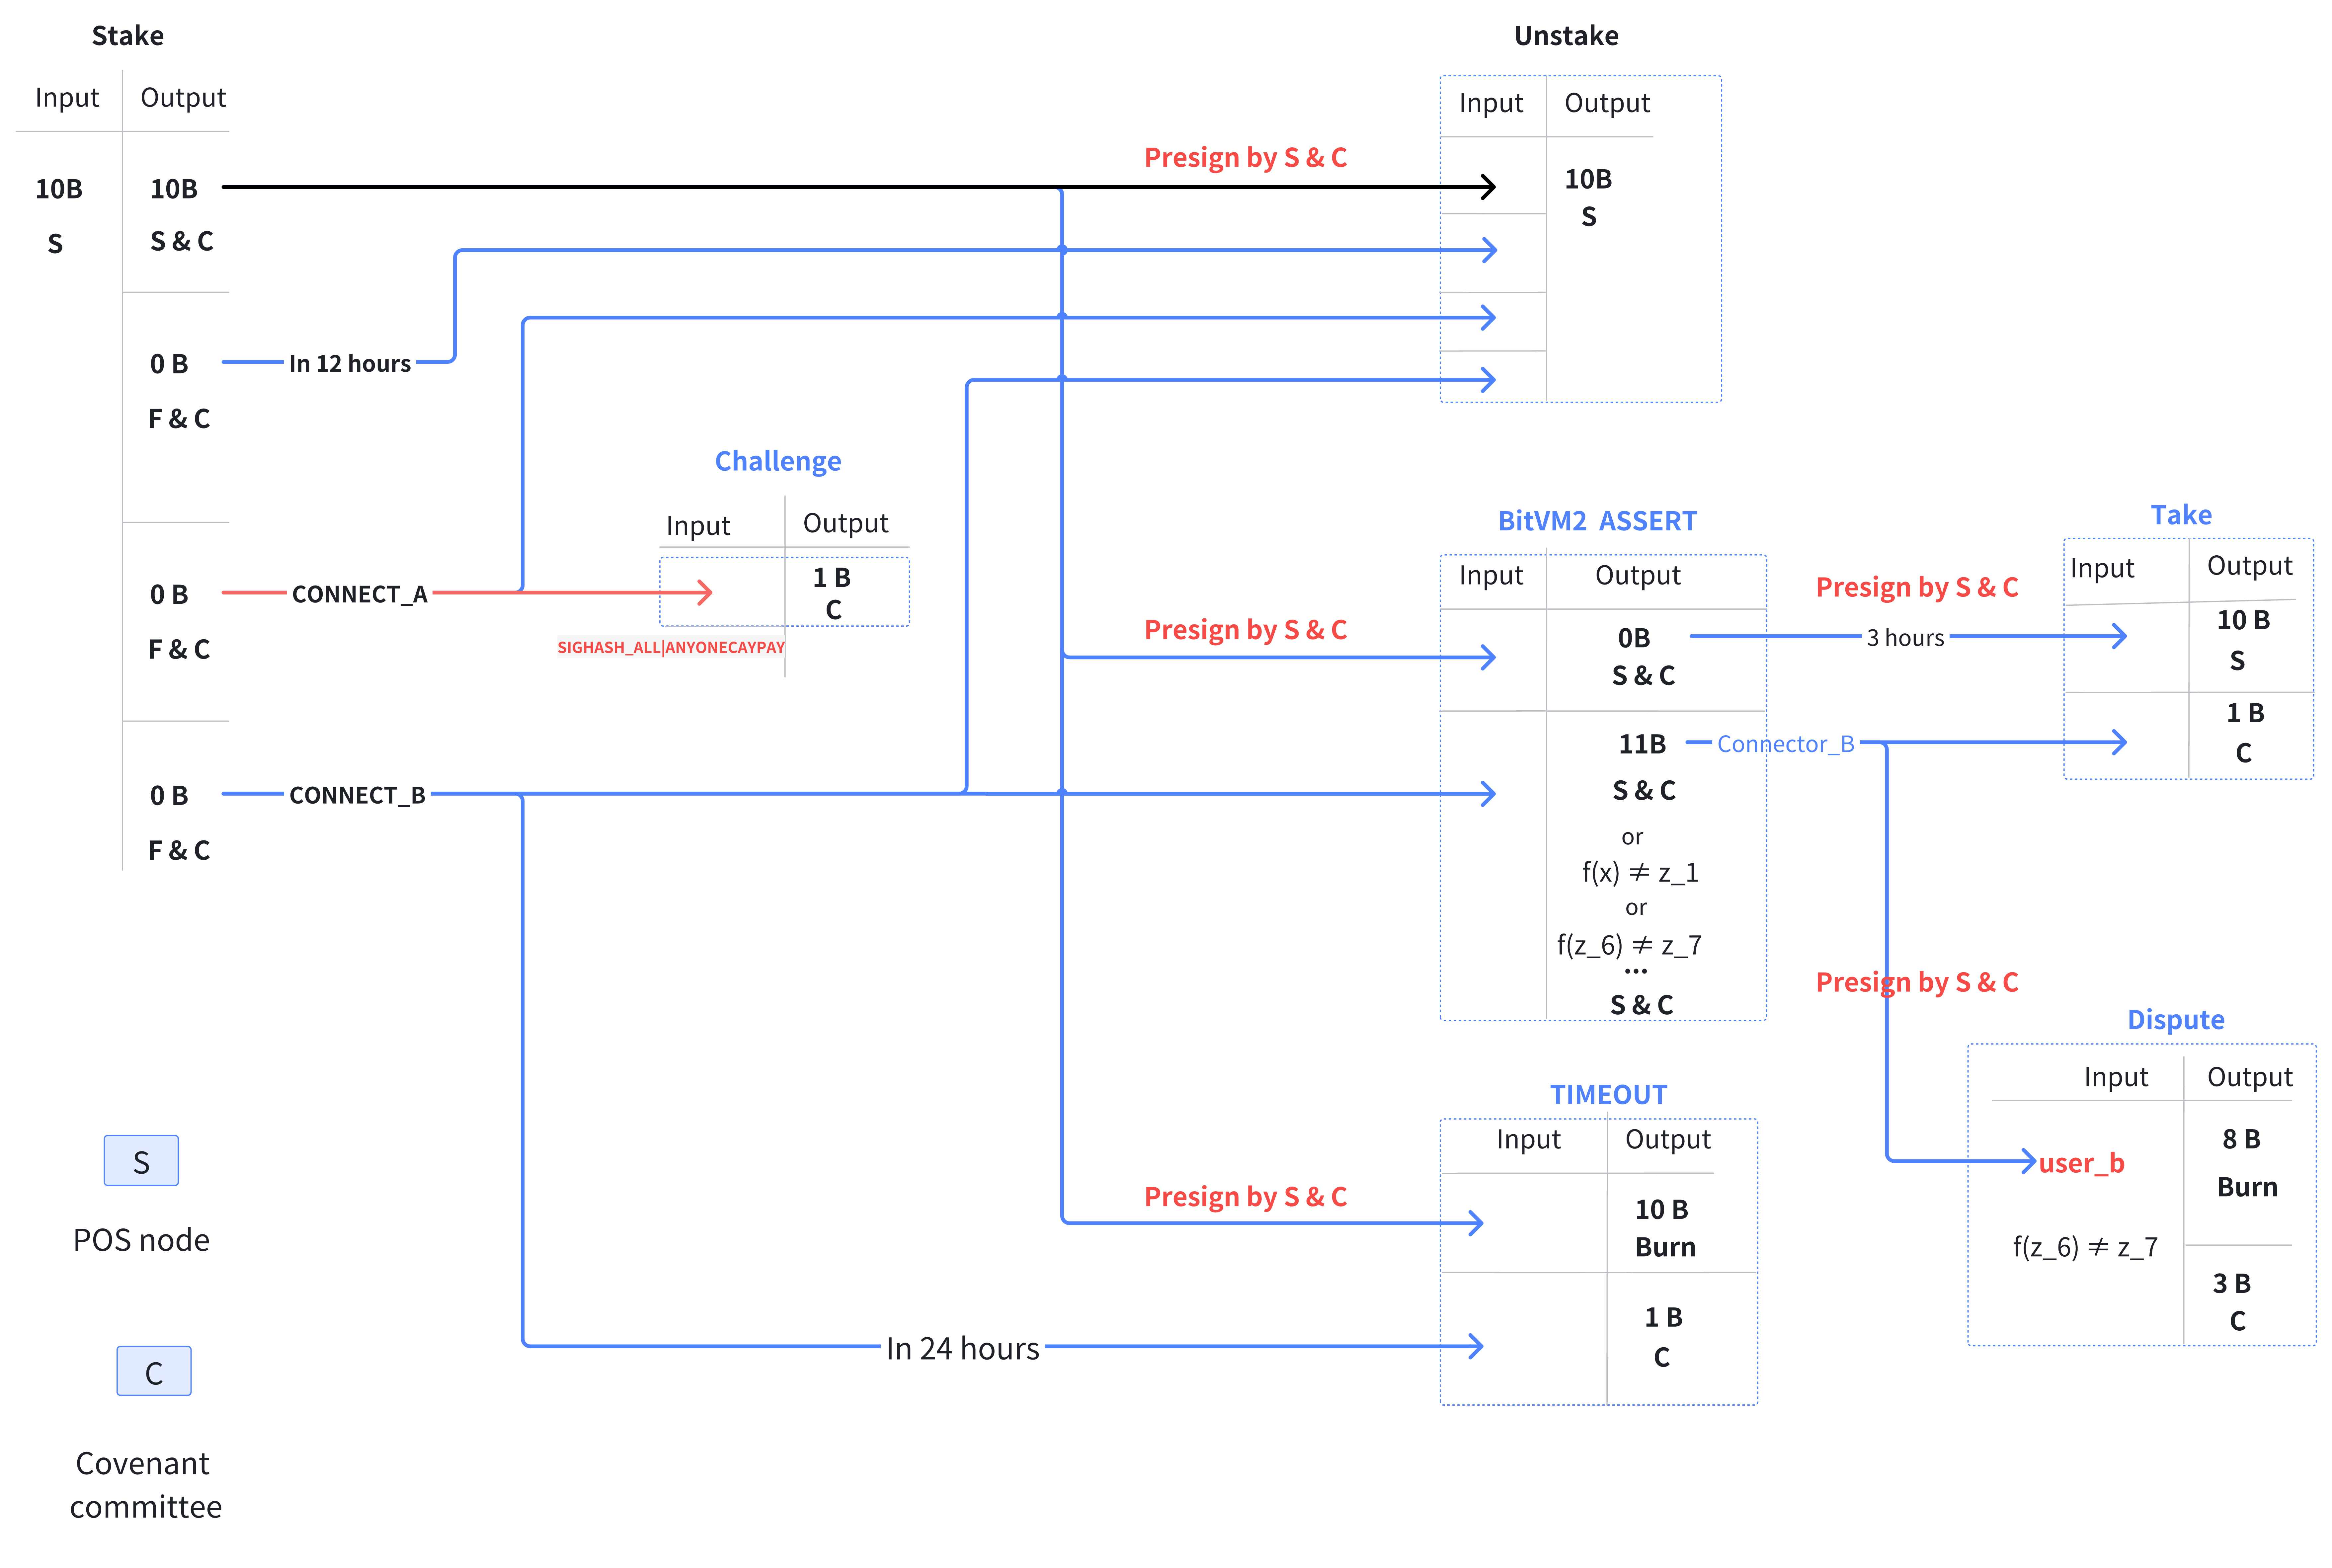
\includegraphics[width=0.85\columnwidth]{images/bitvm2 protocol.png} 
    \caption{bitvm2 protocol}
    \label{fig:bitvm2 protocol}
\end{figure}

Now, we will give clear clarification on it with 3 paragraphs

\paragraph{Roles}

We intrduce the roles firstly:

\begin{itemize}
    \item S: The staker, The guys who stake BTC as a POS node in Fiamma
    \item C: The Committee, which is made up of important partners of Fiamma
    \item Challenger: The guy who is willing to kick-off the challenge by paying 1 BTC
    \item user\_b: The guy who kick off the dispute transaction on Bitcoin 
\end{itemize}

\paragraph{Transactions}

We intrduce the function of each transaction:

\begin{itemize}
    \item Stake transaction: Somebody stakes e.g 5 BTC as a POS node of Fiamma by issuing a Stake transaction
    \item Unstake transaction: S could take the staking asset at anytime by issuing a Unstake transaction
    \item Challenge transaction: Challenger could kick off the Challenge transaction by paying 1 BTC, It should be noted that Challenger is permissionless
    \item Assert transaction: Generate a taproot address and then tranfer the staking BTC to taproot address, anyone could spend this taproot address if he can provide a valid witness of any leaf
    \item Take transaction: Take the staking BTC back to S if nobody can spend the taproot address in a fixed time, the Challenger lose 1 BTC
    \item Dispute transaction: Anyone could kick off this transaction if he can spend the taproot address, the S will be slashed
    \item Timeout transaction: If challenge happens, S still could be slashed if the Assert transaction does not be kicked off in a fixed time
\end{itemize}

\paragraph{Overall flow}

We will give the overall flow of the whole protocol as the following picture:

\begin{figure}[ht] 
    \centering  
    \includegraphics[width=0.85\columnwidth]{images/bitvm2 simple flow.png} 
    \caption{bitvm2 simple flow}
    \label{fig:bitvm2 simple flow}
\end{figure}

\begin{itemize}
    \item S stake e.g 5 BTC as a POS node of Fiamma
    \item S pre-sign 6 transactions with Committee at the initial phase (We should stop S provides service if he doesn't sign these 6 transactions)
    \item S provides ZKP verification service in Fiamma chain and store the inputs, outputs, and all immediate vaules in POS chain as well as the Winternitz signature for these values;
    \item At the phase, the proof state is soft finality which means that it's secured by POS network until Now
    \item The intersubjective nodes in Fiamma will actively to monitor the POS chain and access to the proof which its state is soft
    \item When the proof get enough number of confirmation, e.g exceed the threshold, the proof state move to hard finality
    \item Only if one of intersubjective nodes is honest, he will find S give a wrong claim, then he kick the Challenge transaction
    \item S broadcast the Assert transaction
    \item Anyone (user\_b) will kick off the Dispute transactions, normally, user\_b is the Challenger
    \item Then S is slashed
    \item If the Dispute transaction doesn't be broadcast after a fixed time, S take asset back by issuing the Take transactions
\end{itemize}

\subsubsection{Core features}

Our protocol have several nice properties as follows:

\begin{itemize}
    \item Trustless for asset security: The asset is safe and there doesn't introduce any additional assumption
    \item Trust-minimized for protocol: if S is malicious, S will be slashed only if one of intersubjective nodes is honest
    \item Decentralized for network: As intersubjective nodes is permissionless, so the protocol is decentralized enough and also safe enough
    \item Nice economic game: S and intersubjective nodes wouldn't love to be malicious becasue of the punish machanism. nodes would love to challenge if S is malicious because of the potential reward
\end{itemize}

\subsubsection{To be improved and completed}

The protocol we describe before is an ideal case, there still have a few points to be moted, improved, and completed

\begin{itemize}
    \item BTC slashing: Because Babylon only support double sign fault, the POS node have to stake additional BTC to correspond to validity fault. It will be improved when Fiamma help Babylon integrate BitVM2 part;
    \item Taproot address generation: The subscript number of MSM is dynamic as the coefficient is different for different proof 
    \item Reward delivery: It cannot know ahead who will be the Challenger at initial phase, so the Committee will responsible for this part
    \item Security: The protocol is definitely safe and works only if S and C won't be malicious at the same time
    \item Staking for intersubjective nodes: The intersubjective nodes have to stake some asset on Fiamma or Bitcoin in case they are out of service or malicious
    \item On-chain cost for challenge process: As we don't need to store the data and commitments on Bitcoin, we should keep reduce the size of all subscripts to save the challenge cost
    \item Blake3 Hash integrate: We will complete blake3 hash part for Winternitz \cite{website:witernitz} signature;
    \item Winternitz signature: We ill completed this part at next step
\end{itemize}
